\section{Si descriva cos'è la tecnica del selective repeat}

Il problema di ricezione dell'ack per ogni frame inviato limitava di molto l'utilizzo della banda e rallentava le comunicazioni.
Per ovviare a questo problema viene usata la tecnica di pipelining.
Si decide quindi di inviare più frame prima di ricevere i vari ack aumentando di parecchio l'utilizzo della linea.
Tuttavia, sorge un problema: cosa succede nel caso in cui si perdano dei frames?
Per il ripristino degli errori in presenza di pipelining sono disponibili due approcci base: selective repeat e go back-n.
\subsection{Cos'è?}
Con il selective repeat, quando viene ricevuto un frame in errore viene scartato, mentre i frame buoni ricevuti successivamente vengono salvati in un buffer;
quando la sorgente va in timeout, solo il frame più vecchio senza ACK viene ritrasmesso.
Se quel frame arriva correttamente, la destinazione può passare in sequenza allo strato network tutti i frame presenti nel buffer.

La ripetizione selettiva può inviare dei NACK (Not acknowledgement) quando trova un errore, così da stimolare la ritrasmissione prima dello scadere del timer.
La ripetizione selettiva corrisponde ad avere una finestra di ricezione maggiore di 1.

Go back-n e il selective repeat hanno diverse conseguenze in termini di uso di banda e di spazio di buffer nello strato data link.
Si può utilizzare un approccio o l'altro in base a quale risorsa è più scarsa.

\begin{figure}[H]
\centering
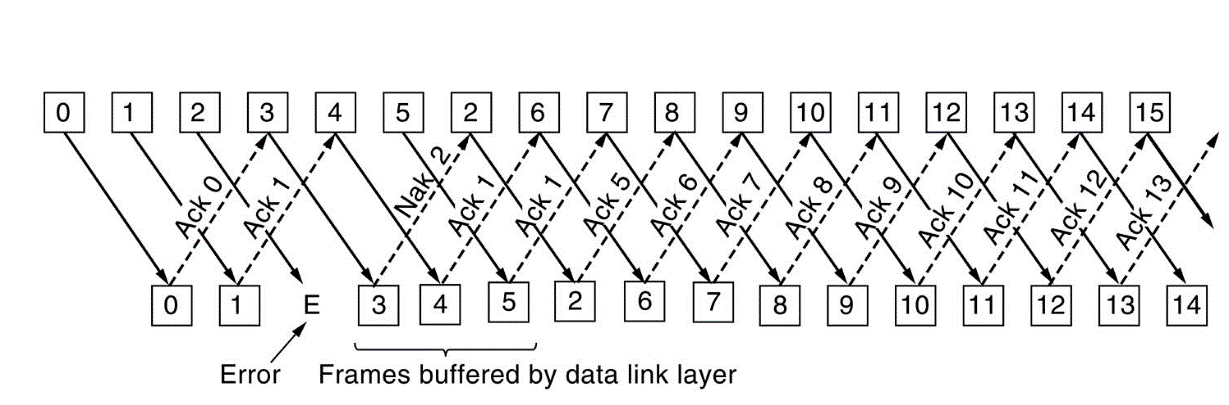
\includegraphics[scale=0.8]{res/img/21_SelectiveRepeat.png}
\end{figure}
 
\subsection{Pregi}
Aumentano di molto le performance, soprattutto grazie ai NACK che stimolano la ritrasmissione prima dello scadere del timer.

\subsection{Difetti}
Essendo una ricezione non sequenziale c'è il rischio che gli intervalli della prima finestra si sovrappongano con la successiva, con conseguenza che il ricevitore non sa' se siano dati ritrasmessi (se gli ACK vengono persi) o dati nuovi (se gli ACK sono stati ricevuti).

\subsection{Ambiti d'uso}
Utilizzato in base alla disponibilità delle risorse, finestra di ricezione maggiore di 1.

\section{Descrivere la differenza tra ALOHA e ALOHA-SLOTTED}
\subsection{Cos'è ALOHA?}
ALOHA è un protocollo di rete per garantire le funzionalità di accesso multiplo al mezzo di trasmissione dati condiviso tra più utenti.
Esistono due tipi di reti: quelle che utilizzano le connessioni punto-punto e quelle che usa canali broadcast;
questo protocollo viene utilizzato per le seconde.

Inventato negli anni '70 nelle Hawaii, l'idea di fondo è di consentire agli utenti di trasmettere ogni volta che hanno dati da inviare.
Questo naturalmente genera collisioni, tuttavia i canali broadcast danno la possibilità di avere il feedback sul frame trasmesso e  verificare se il frame è stato ricevuto correttamente o no;
la stazione trasmittente ascolta il canale e determina il successo o insuccesso della trasmissione.
Se il frame viene danneggiato, le stazioni aspettano un tempo casuale prima di ritrasmettere (deve essere casuale altrimenti i frame si danneggiano continuamente).
Il successo dell'ALOHA puro è di circa 18\%.

\subsubsection{Pregi}
Permette l'accesso multiplo allo stesso mezzo di trasmissione condiviso da più utenti (broadcast). (pregio?)

\subsubsection{Difetti}
Poco efficiente in comunicazioni con tante stazioni.

\subsubsection{Ambiti d'uso}
Protocollo di livello MAC, questo protocollo non è attualmente utilizzato.
Creato tuttavia per l'utilizzo nelle connessioni di tipo broadcast, in cui il mezzo trasmissivo è condiviso da più di due punti.

\subsection{Cos'è ALOHA Slotted?}
Il protocollo Slotted ALOHA aggiunge al protocollo sopracitato la divisione del tempo in intervalli discreti, chiamati slot.
Ogni stazione viene vincolata a cominciare la propria trasmissione solo all'inizio di uno slot temporale,
se una stazione è pronta a trasmettere, dovrà necessariamente attendere l'inizio dello slot successivo.

Lo svantaggio di questo protocollo è la necessità di un meccanismo di sincronizzazione che indichi alle varie stazioni quando possono cominciare la trasmissione.
Questa divisione in slot migliora il grado di successo del doppio rispetto all'ALOHA puro, circa 36\%.

Questi risultati non dovrebbero sorprendere, in quanto con stazioni che trasmettono a piacimento è molto facile incorrere in collisioni.

Questi protocolli caddero in disuso, fino a quando non si presentò il problema di allocare un canale condiviso da più utenti in competizione
(ad esempio dopo l'invenzione dell'accesso ad Internet via cavo), di conseguenza slotted ALOHA tornò ad essere utilizzato.

\subsubsection{Pregi}
Migliora l'ALOHA puro, aumentando il grado di successo di circa il doppio.

\subsubsection{Difetti}
Necessita di un meccanismo di sincronizzazione che indichi alle varie stazioni quando trasmettere.

\subsubsection{Ambiti d'uso}
Protocollo di livello MAC, utilizzato nelle connessioni broadcast per condividere lo stesso mezzo trasmissivo da più utenti.

\begin{figure}[H]
\centering
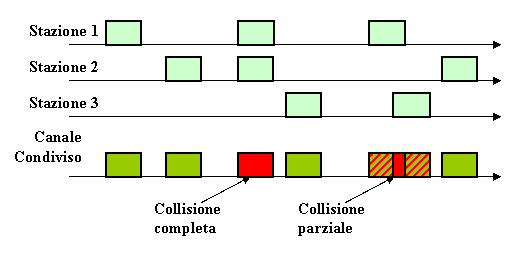
\includegraphics[scale=0.7]{res/img/22_ALOHA.png}
\end{figure}
\begin{figure}[H]
\centering
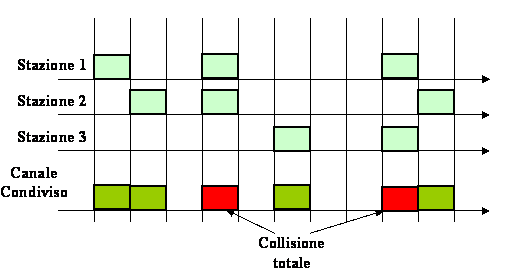
\includegraphics[scale=0.7]{res/img/22_ALOHASLOTTED.png}
\end{figure}

\section{Si illustri il CSMA (Carrier Sense Multiple Access), indicandone pregi e difetti}

I protocolli ALOHA e le sue varianti permettevano di inviare dati ogniqualvolta si voleva, limitando però le percentuali di successo.
Per migliorare i risultati di accesso multiplo ad un mezzo di trasmissione condiviso, vengono implementati protocolli in cui le stazioni rimangono in ascolto di una portante e si comportano di conseguenza. Questi protocolli sono chiamati protocolli con rilevamento della portante.
\subsection{Cos'è?}
Il CSMA è una tecnica di trasmissione dati che si basa su questi principi.
Ogni dispositivo prima di avviare la trasmissione dei dati deve verificare se altri nodi stanno trasmettendo sul canale, rilevando la portante.
Se il canale è libero iniziano a trasmettere, altrimenti attendono un tempo arbitrario prima di riprovare.
Esistono diverse versioni di CSMA:
\begin{itemize}
\item	CSMA 1-persistente: è il primo tra i protocolli CSMA, ha la particolarità di inviare con probabilità 1 sul canale in caso di nessun rilevamento.
Questo migliora sicuramente ALOHA puro, tuttavia l'ingordigia di inviare non appena si libera il canale non rende immuni dalle collisioni, che potrebbero accadere in caso di stazioni che controllano nello stesso momento un canale vuoto e inviano contemporaneamente.
\item	CSMA non persistente: prima di trasmettere ogni stazione controlla il canale.
Se lo trova libero inizia ad inviare i dati, ma se il canale è occupato la stazione non esegue un controllo continuo per trasmettere subito il proprio frame;
invece attende per un intervallo casuale prima di ripetere l'algoritmo. Questo meccanismo permette di utilizzare meglio il canale ma allunga i ritardi.
\item	CSMA p-persistente: questa variante si applica su canali divisi in intervalli temporali.
Quando è pronta a trasmettere, ogni stazione controlla il canale.
Se lo trova libero, trasmette subito con una probabilità p, e rimanda fino all'intervallo successivo con probabilità q=1-p.
Se anche quell'intervallo risulta libero la stazione trasmette oppure rimanda un'altra volta. Il processo si ripete finché il frame non è stato trasmesso.
\end{itemize}
Queste varianti migliorano enormemente il tasso di successo rispetto ad ALOHA e ALOHA-slotted.

Un ulteriore miglioramento si ottiene consentendo ad ogni stazione di annullare la propria trasmissione in caso di collisione.
Se due stazioni iniziano a trasmettere contemporaneamente, invece di completare la trasmissione dei relativi frame, ormai danneggiati, terminano bruscamente la trasmissione.
La terminazione rapida dei frame danneggiati risparmia tempo e banda, questa variante è chiamata CSMA/CD ed è ampiamente utilizzata nelle LAN Ethernet.

\begin{figure}[H]
\centering
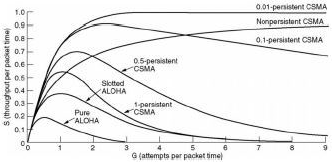
\includegraphics[scale=1]{res/img/23_CSMA.png}
\end{figure}

\subsection{Pregi}
Migliora di molto le prestazioni di ALOHA e ALOHA-SLOTTED, un ulteriore miglioramento si ha quando si annulla la propria trasmissione in caso di collisione, cosi da risparmiare tempo e banda.

\subsection{Difetti}
--

\subsection{Ambiti d'uso}
CSMA/CA è utilizzato prevalentemente nelle connessioni in cui il rilevamento delle collisioni non è realizzabile, come le reti senza fili.
Utilizzato nello standard IEEE 802.11.
Una variante migliorante, che rileva le collisioni è il CSMA/CD il quale è utilizzato nelle LAN Ethernet.

\section{Basic Bitmap}

Nella gestione di accesso multiplo ad un mezzo di trasmissione condiviso, esistono diversi protocolli che gestiscono l'accesso gestendo le collisioni e garantendo l'accesso (ALOHA, slotted ALOHA, CSMA), tuttavia le collisioni sono sfavorevoli alle prestazioni del sistema, specialmente quando il cavo è lungo e i frame corti.
\subsection{Cos'è?}
Esistono protocolli che garantiscono la gestione degli accessi senza collisione, uno tra questi è il basic Bitmap (metodo a mappa di bit elementare). In questo protocollo ogni periodo di contesa è composto esattamente da N intervalli (N=\# stazioni). Ogni stazione è numerata, e se ha un frame da inviare deve inviare un “1” nell'intervallo corrispondente al suo numero. A nessun'altra stazione è concesso di trasmettere durante questo intervallo. Cosi facendo ogni stazione si “prenota” l'intervallo di trasmissione. Una volta trascorsi gli N intervalli, ogni stazione sa quali sono le stazioni che vogliono trasmettere, di conseguenza non ci sarà mai alcuna collisione.
Questo è anche chiamato protocollo a prenotazione.

\subsection{Pregi}
Garantisce che non ci siano collisioni durante l'utilizzo di un canale condiviso.

\subsection{Difetti}
Protocollo sbilanciato, da priorità alle stazioni con un numero basso, se una stazione “i” e una “j” vogliono trasmettere e i<j allora i si aggiudica la posizione.\\
Contemporaneamente però le stazioni numerate con numeri bassi dovranno attendere di più rispetto a quelle con numeri più alti.\\
Ha bisogno di 1 bit di controllo per stazione, in reti con migliaia di utenti non è molto adatto.

\subsection{Ambiti d'uso}
Protocollo dello strato MAC, utilizzato nelle connessione con canale condiviso

\section{Spiegare in cosa consiste il protocollo collision free binary countdown, pregi e difetti}

I dati vengono trasportati tramite un impulso elettrico. Ci possono essere molti dispositivi collegati allo stesso cavo con il rischio di collisioni e danneggiamento dei dati.
Per evitare la collisione una stazione deve controllare se ci sono altre stazioni collegate allo stesso mezzo; esistono diversi protocolli che effettuano questo controllo evitando le collisioni.
Il basic bitmap è uno di questi, tuttavia risulta elementare e su reti composte da molte stazioni risulta poco utilizzabile.

\subsection{Cos'è?}
Il collision free binary countdown o conteggio binario migliora il basic bitmap, utilizzando un sistema di assegnazione della linea in base ad una stringa binaria.
Una stazione che desidera utilizzare il canale deve comunicare a tutti il proprio indirizzo sotto forma di stringa binaria, hanno tutti la stessa lunghezza.

I conflitti si evitano grazie ad una regola di arbitraggio: la stazione rinuncia ad inviare non appena si accorge che un'altra stazione con un “1” in una posizione di bit di ordine elevato che nel proprio indirizzo vale “0”.
Esempio: 0010, 0100, 1001, 1010, queste stazioni vogliono inviare, vengono inviati i primi bit: 0 (\textbf{0}010), 0 (\textbf{0}100), 1 (\textbf{1}001), 1 (\textbf{1}010), le stazioni con “0” più a sinistra capiscono che ci sono stazioni con numero più grande che stanno concorrendo e si fanno da parte, le altre due continuano: 0 (1\textbf{0}01), 0 (1\textbf{0}10); sono uguali quindi continuano, il terzo bit è “1” quindi la stazione 1001 si arrende, vince 1010 che può trasmettere.

L'efficienza è pari a ($d/d*log_2N$) (con d numero di bit) ma può raggiungere anche il 100\% se l'indirizzo del mittente costituisce l'intestazione del frame.

Si può notare uno sbilanciamento notevole in quanto le stazioni con numero maggiore risultano avere sempre la precedenza. Questo può essere ovviato facendo ruotare i valori delle stazioni ad ogni step, così quando una stazione riesce ad inviare viene spostata alla fine della coda, in modo da permettere a tutte le stazioni la possibilità di inviare.

Questo algoritmo è semplice, elegante ed efficiente, tuttavia attualmente non è utilizzato.

\subsection{Pregi}
Migliora il problema della scarsa efficienza in caso di molte stazioni del basic bitmap.
Garantisce comunicazioni senza collisioni.
Ad alto carico l'efficienza del canale migliora.

\subsection{Difetti}
Da priorità alle stazioni con numero maggiore, con conseguente sbilanciamento. Problema risolto facendo ruotare i valori delle stazioni ad ogni step. 
A basso carico hanno un ritardo elevato.
\subsection{Ambiti d'uso}
Protocollo dello strato MAC. Utilizzato nelle connessione con canale condiviso. Attualmente non utilizzato.

\begin{figure}[H]
\centering
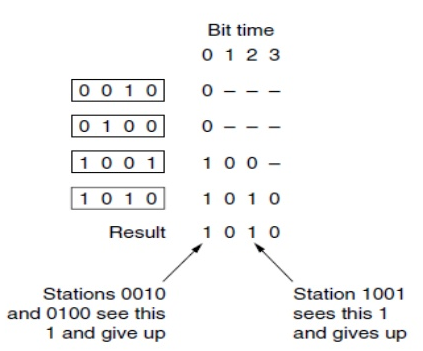
\includegraphics[scale=0.6]{res/img/25_FreeBinaryCountdown.png}
\end{figure} 

\section{Spiegare cos'è l'adaptive tree walk protocol?}

Per gestire la contesa di accesso ad un canale condiviso esistono protocolli con controllo della portante, con metodo della contesa tipo il CSMA o il metodo senza collisioni. Nelle situazioni di carico leggero la contesa è preferibile per il suo basso ritardo, tuttavia a carichi elevati diventa sempre più inefficiente. Il contrario avviene con i protocolli senza collisioni, a basso carico hanno un ritardo elevato ma al crescere del carico l'efficienza migliora.
\subsection{Cos'è?}
Adaptive tree walk protocol è un protocollo a contesa limitata che migliora ulteriormente le prestazioni dei protocolli sopracitati.
Si può immaginare questo metodo come un albero binario, in cui le stazioni sono le foglie e sono divise nei vari rami. Inizialmente si prova a inviare ad altezza 0: se non vi è collisione si procede all'invio, in caso contrario ci si sposta sul sottoalbero sinistro e si ritenta; se il conflitto non c'è più si fa inviare la stazione che lo desidera (se non c'è conflitto vuol dire che nel sottoalbero sinistro c'è solo una stazione che vuole inviare). Dopo aver inviato si torna al nodo padre e si analizza il sottoalbero destro, ripetendo i test e scendendo nei sottoalberi in caso di conflitto.

\begin{figure}[H]
\centering
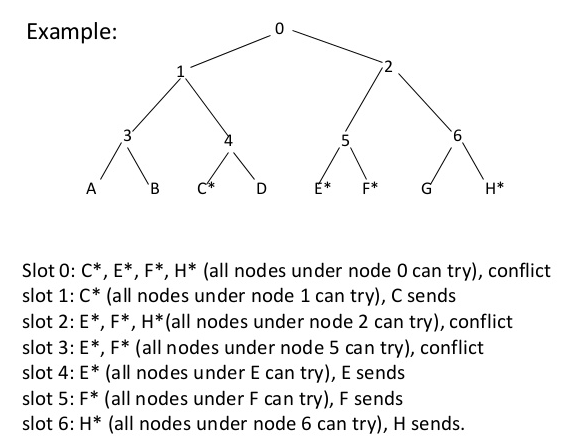
\includegraphics[scale=0.7]{res/img/26_AdaptiveTreeProtocol.png}
\end{figure}

\subsection{Pregi}
Garantisce un ritardo limitato in caso di basso carico e una buona efficienza in caso di carico più elevato.
\subsection{Difetti}
--
\subsection{Ambiti d'uso}
Utilizzato nelle connessioni con più stazioni che vogliono trasmettere nello stesso mezzo di trasmissione.

\section{Ethernet e i vari tipi di cavo}
\subsection{Cos'è?}
Ethernet è il sistema LAN più diffuso al mondo, è economico e facile da usare e la diffusione delle componenti hardware ne ha facilitato l'adozione. È adeguata all'utilizzo con TCP/IP.

Nasce con l'intento di ottenere una trasmissione affidabile su cavo coassiale in condizioni di traffico contenuto, ma in grado di tollerare possibili picchi di carico. Per regolamentare l'accesso al mezzo trasmissivo era stato adottato un protocollo di accesso multiplo del tipo CSMA/CD.

Il nome Ethernet si riferisce al cavo (definito “etere”). Andiamo quindi ad elencare le tipologie di cavi utilizzati in questo standard.
Generalmente vengono utilizzati 4 tipi di cavo.
\subsection{10base5}
Il più vecchio è il modello 10base5 chiamato anche thick Ethernet. Questo cavo assomiglia ad un tubo giallo con segni a intervalli di 2,5m che indicano la posizione delle spine.
Le connessioni sono generalmente realizzate mediante spine a vampiro (spilli spinti nel nucleo centrale del cavo coassiale). 
La notazione 10Base5 indica che opera a 10Mbps, utilizza un sistema di segnali a banda base e può supportare segmenti lunghi fino a 500m. Questo cavo è ormai obsoleto.
\subsection{10base2}
Il secondo cavo in ordine di tempo è stato il cavo 10base2 o thin Ethernet, più facile da piegare rispetto al precedente e le connessioni sono realizzate usando connettori BNC (giunzioni a “T” più affidabili e facili da usare rispetto alle spine a vampiro). Il thin Ethernet è più economico e semplice da installare, però può essere lungo al massimo 185 metri e può supportare non più di 30 macchine.
\subsection{10base-T}
Per trovare guasti in questi mezzi è usata la tecnica TDR (Time Domain Rectory) che sostanzialmente misura il ritardo dell'eco dell'impulso immesso nel cavo.
La tecnica TDR per la ricerca di guasti è difficile e onerosa da utilizzare, ci si è spostati quindi sulla terza tipologia di cablaggio 10Base-T, ormai diventata uno standard grazie alla facilità di gestione e all'uso di cablaggi preesistenti.

Questo sistema di cablaggio utilizza hub di controllo tramite doppini telefonici, che sono largamente usati e semplici da gestire, ogni macchina si interfaccia con l'hub tramite cavo dedicato, rendendo così semplice aggiungere o rimuovere una stazione e individuare le interruzioni. Il suo svantaggio è rappresentato dalla lunghezza massima dei cavi che partono dall'hub: 100 metri. Esiste una versione più veloce del 10Base-T chiamata 100Base-T.
\subsection{10base-F}
Il quarto tipo di cavi per Ethernet si chiama 10base-F e utilizza le fibre ottiche. È un'alternativa costosa a causa del prezzo dei connettori e dei terminatori, ma offre un'eccellente immunità alle interferenze e consente di collegare edifici o hub molto lontani. 10Base-F nonostante il costo consente inoltre una buona sicurezza in quanto i dati trasmessi sulla fibra sono difficili da intercettare.
 
\begin{figure}[H]
\centering
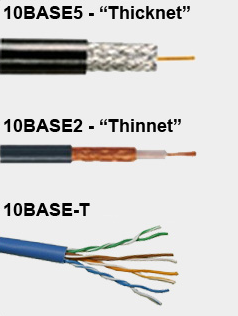
\includegraphics[scale=0.6]{res/img/27_CaviEthernet.png}
\end{figure}

\subsection{Pregi}
Sistema LAN più diffuso, economico e facile da utilizzare.
I primi due tipi di cavo non vale la pena analizzarli perchè ormai sono obsoleti, i 10base-T sono sicuramente più economici rispetto ai 10base-F che tuttavia provvedono a garantire un'eccellente immunità alle interferenze e una velocità molto superiore alla controparte in rame.
Grazie all'utilizzo degli hub i guasti sono semplici da localizzare e correggere.

\subsection{Difetti}
I 10base-T hanno una lunghezza massima molto limitata: 100 metri dall'hub.
I 10base-F costano molto.

\subsection{Ambiti d'uso}
I primi due non sono utilizzati, il 10base-T è diventato una tipologia standard di cablaggio nello standard Ethernet, i 10base-F vengono utilizzati largamente in tutte le nuove reti ad alta velocità.

\section{Codifica Manchester}

Nessuna versione Ethernet usa la pura conversione binaria dov il del segnale “0” viene indicato con 0 volt mentre “1” utilizzando 5 volt. Questo fa sorgere numerosi problemi, in quanto altre stazioni potrebbero interpretare erroneamente il segnale (a causa degli 0 volt, una stazione potrebbe confondere l'assenza del segnale con uno “0”). Si può passare a +1 volt per “1” e -1 volt per “0”, ma rimane il problema dei ricevitori che possono campionare il segnale in maniera diversa.
Per risolvere questo problema sono state inventate due tecniche implementate in Ethernet: codifica Manchester e codifica Manchester differenziale.
\subsection{Codifica Manchester cos'è?}
Queste codifiche sono dette auto-sincronizzanti in quanto non necessitano di un segnale di sincronia esterno.
Queste codifiche suddividono ogni bit codificato in due, nella codifica Manchester lo “0” viene rappresentato da un segnale Basso-Alto, mentre l'”1” viene rappresentato da un segnale Alto-Basso (esistono due convenzioni opposte riguardo la rappresentazione dei segnali “1” e “0”).
Così facendo anche in caso di dissincronia, i dati in questo formato permettono un flusso auto-sincronizzante. Uno svantaggio e' che la codifica manchester richiede il doppio della banda rispetto alla pure conversione binaria 0-5 volt.
\subsection{Codifica Manchester differenziale cos'è?}
La codifica Manchester differenziale invece differisce da quella originale nella rappresentazione dei bit: questa infatti si basa sulla verifica di transizioni all'inizio di un intervallo. La presenza di una di queste infatti (che siano alto-basso o basso-alto) identifica un valore, la mancanza di transizione invece indica il valore opposto. Per convenzione il bit 1 viene rappresentato dalla mancanza di transizione all'inizio del suo intervallo, mentre lo 0 è indicato con un cambiamento di segnale nello stesso periodo. Rispetto a manchester normale, la codifica differenziale e' piu' complessa a livello hw ma offre migliori prestazioni per quanto riguarda il disturbo di segnale.

\begin{figure}[H]
\centering
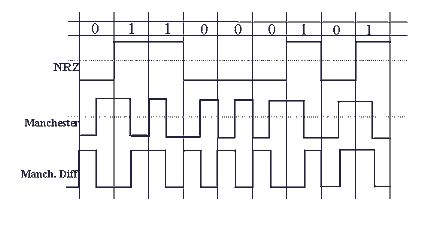
\includegraphics[scale=0.8]{res/img/28_CodificaManchester.png}
\end{figure}

\subsection{Pregi}
Si risolve il problema di ambiguità dovuto al segnale 0 volt=bit 0.\\
Queste codifiche permettono l'auto sincronizzazione del segnale.

\subsection{Difetti}
Occupano il doppio della banda della codifica binaria elementare, perchè gli impulsi sono larghi la metà.

\subsection{Ambiti d'uso}
Tutti i sistemi Ethernet adottano la codifica Manchester perché è più semplice, mentre la Manchester differenziale è utilizzata da altre LAN.

\section{Cos'è il binary exponential backoff?}
La caratteristica principale del CSMA/CD (algoritmo che controlla il canale prima di trasmettere ed evita le collisioni analizzando la portante) è che una volta rilevata una collisione, si attende un intervallo prima di ritrasmettere. Questo intervallo viene calcolato ogni volta tramite l'algoritmo di backoff esponenziale.

\subsection{Cos'è?}
Dopo una collisione il tempo viene diviso in intervalli discreti, la cui lunghezza è uguale al tempo di propagazione di andata e ritorno del caso peggiore sul mezzo di trasmissione.
Dopo la prima collisione, ogni stazione aspetta 0 o 1 intervalli temporali prima di ritentare. Se due stazioni collidono e ognuna sceglie lo stesso numero casuale, la collisione si ripeterà. Dopo la seconda collisione ogni stazione sceglie 0, 1, 2 o 3 a caso e rimane in attesa per quel numero di intervalli temporali. In generale quindi, dopo le collisioni, viene scelto un numero casuale compreso tra 0 e 2i-1 e si salta quel numero di intervalli. Il limite di collisioni è 16, dopodiché il chip di controllo getta la spugna e manda un errore.

\subsection{Pregi}
Si adatta dinamicamente al numero di stazioni che tentano di trasmettere.\\
Assicura un basso ritardo quando poche stazioni collidono e garantisce un intervallo di tempo ragionevole quando invece la collisione coinvolge molte stazioni

\subsection{Difetti}
--

\subsection{Ambiti d'uso}
Utilizzato nel protocollo di accesso multiplo CSMA/CD, e serve per decidere/calcolare il tempo di entrata di una stazione nel canale (dopo una collisione).
\section{Stazione nascosta e stazione esposta: cosa sono e cosa fanno?}

Al crescere del numero di computer e dispositivi mobili aumenta anche la domanda di collegare tali apparecchi al mondo esterno.
Nascono così le LAN wireless, le quali permettono la connessione dei dispositivi senza bisogno di cavi.

Tuttavia, questo porta a dei problemi di conflitto in caso di scambio di dati.
Utilizzando banalmente il sistema CSMA per evitare le collisioni, si arriverebbe ad ascoltare le altre trasmissioni, e trasmettere in caso di nessun'altra connessione attiva.
Questo però può portare a due diversi problemi: problema della stazione nascosta e stazione esposta.
\subsection{Stazione nascosta, cos'è?}
La stazione nascosta non è altro che una stazione che vuole inviare, ma non riesce a ricevere i segnali dei concorrenti a causa della sua distanza eccessiva. Supponiamo di avere A, B e C. A vuole inviare a B e prima di farlo ascolta se ci sono altre connessioni; non ne sente e procede all'invio. Tuttavia, C, è troppo distante perché A lo senta, ma abbastanza vicino a B per inviargli dati, così lo fa e va in conflitto con l'invio di A.

\begin{figure}[H]
\centering
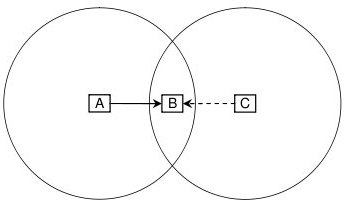
\includegraphics[scale=0.6]{res/img/30_StazioneNascosta.png}
\end{figure} 

\subsection{Stazione esposta, cos'è?}

Il problema della stazione esposta invece è l'inverso. B trasmette ad A, C vuole inviare a D e controlla la presenza di portante sul mezzo di trasmissione e rileva B che sta inviando, così attende per evitare conflitti; tuttavia B non intralcerebbe la trasmissione di C, ma questo non lo può sapere, di conseguenza si genera uno stallo inutile. Questo è il problema della stazione esposta.
 
 \begin{figure}[H]
\centering
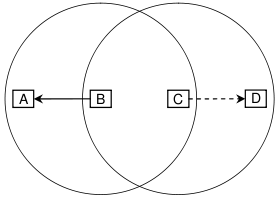
\includegraphics[scale=0.6]{res/img/30_StazioneEsposta.png}
\end{figure} 
